\documentclass[12pt]{article}
\usepackage[margin=1in]{geometry}
\usepackage{graphicx}
\usepackage{booktabs}
\usepackage{array}
\usepackage{longtable}
\usepackage{hyperref}
\usepackage{caption}
\usepackage{float}
\usepackage{titlesec}
\usepackage{enumitem}
\usepackage{parskip}
\usepackage{fancyhdr}
\usepackage{xcolor}

\hypersetup{
    colorlinks=true,
    linkcolor=black,
    urlcolor=blue
}

\pagestyle{fancy}
\fancyhf{}
\rhead{CS 4632 -- Milestone 5}
\lhead{Munir Gargour}
\rfoot{\thepage}

\graphicspath{{output/}{./}}

\title{
    \textbf{CS 4632: Modeling and Simulation}\\
    \large Milestone 5: Final Report\\[0.5em]
    \normalsize Seasonal Predator-Prey Simulation
}
\author{Munir Gargour}
\date{\today}

\begin{document}

\begin{titlepage}
    \centering
    \vspace*{2cm}
    
    {\Huge\bfseries Seasonal Predator-Prey Simulation\par}
    \vspace{1.5cm}
    {\Large\itshape Final Report\par}
    \vspace{2cm}
    {\Large\bfseries Munir Gargour\par}
    \vfill
    {\large CS 4632: Modeling and Simulation\par}
    {\large Department of Computer Science\par}
    {\large Kennesaw State University\par}
    \vspace{1cm}
    {\large \today\par}
    \vspace{1.5cm}
    {\large \textbf{GitHub Repository:} \url{https://github.com/munirgargour/seasonalpredatorprey}\par}
\end{titlepage}

\begin{abstract}
This report details the design, implementation, and analysis of a continuous 2D agent-based simulation of seasonal predator-prey dynamics. Building upon classic Lotka-Volterra models, this project introduces spatial constraints and seasonal variation to explore how these factors influence population stability and cyclic behaviors. The simulation models rabbits (prey), foxes (predators), and grass (resource) on a toroidal plane, utilizing KD-Trees for efficient spatial queries. Ten distinct scenarios were simulated to analyze the effects of initial populations, resource abundance, and seasonal severity. Key findings demonstrate that while classical delayed oscillations emerge naturally from the agent interactions, stable coexistence is highly sensitive to seasonal harshness. The simulation framework proved robust and scalable, providing a comprehensive tool for exploring ecological dynamics.
\end{abstract}

\newpage
\tableofcontents
\newpage

% =============================================================================
\section{Introduction}
% =============================================================================

\subsection{Problem Motivation}
Understanding the dynamics of predator and prey populations is a foundational challenge in ecology. While traditional differential equation models (such as Lotka-Volterra) provide high-level insights, they often assume perfectly mixed populations and constant environmental conditions. Real-world ecosystems feature spatial constraints, localized interactions, and seasonal environmental changes that significantly alter population trajectories. This project aims to simulate these complexities using an agent-based model to observe emergent macroscopic behaviors from microscopic rules.

\subsection{Research Questions}
\begin{itemize}
    \item How do seasonal variations in resource regeneration and metabolic costs affect the stability of predator-prey cycles?
    \item Does replacing a discrete grid-based environment with a continuous 2D spatial plane alter the expected population dynamics?
    \item Can localized vision and individual foraging strategies produce the classic boom-bust cycles observed in theoretical models?
\end{itemize}

\subsection{Project Objectives}
The primary objective of this project is to build a highly configurable, agent-based seasonal predator-prey simulation. Specific goals include implementing hunger-driven foraging and predator pursuit algorithms, simulating a four-season cycle with varying environmental constraints, and developing a robust data collection and visualization pipeline to analyze the resulting dynamics.

\subsection{Report Organization}
This report is organized as follows: Section 2 covers the background and literature review. Section 3 details the model design and architecture. Section 4 describes the implementation. Section 5 outlines the experimental setup, followed by the results and analysis in Section 6. Section 7 discusses validation and verification. Finally, Section 8 provides a discussion of the findings, and Section 9 concludes the report with reflections and future work.

% =============================================================================
\section{Background and Literature Review}
% =============================================================================

\subsection{Theoretical Foundation}
The theoretical foundation of this simulation lies in the Lotka-Volterra equations, which describe the dynamics of biological systems in which two species interact, one as a predator and the other as prey. The model predicts out-of-phase oscillations in population sizes. However, standard Lotka-Volterra models lack spatial dimensions and individual-level behaviors.

\subsection{Related Work}
Agent-based models (ABMs) have been extensively used to study ecological systems. NetLogo's Wolf-Sheep Predation model is a classic example of grid-based predator-prey simulation. This project builds upon such grid-based models by transitioning to a continuous 2D space, allowing for more realistic movement and spatial interactions.

\subsection{Mathematical Models Used}
Instead of relying on global differential equations, this simulation uses discrete-time localized rules. The probability of survival and reproduction for each agent is a function of its accumulated energy, which is affected by its base metabolism, movement cost, and energy gained from consumption. Seasonal multipliers adjust these costs and the environment's carrying capacity dynamically.

\subsection{Justification for Approach}
An agent-based approach in a continuous space, accelerated by KD-Trees, was chosen to overcome the artificial artifacts of grid-based movement (e.g., Manhattan distance limitations). This allows for a more natural representation of pursuit and evasion, and provides a scalable framework for adding more complex sensory and behavioral rules in the future.

% =============================================================================
\section{Model Design and Architecture}
% =============================================================================

\subsection{Conceptual Model}
The simulation represents a closed ecosystem on a toroidal 500x500 continuous spatial plane. It consists of:
\begin{itemize}
    \item \textbf{Grass (Resource):} Regenerates seasonally and provides energy to prey.
    \item \textbf{Rabbits (Prey):} Consume grass, evade predators (implicitly through survival), and reproduce.
    \item \textbf{Foxes (Predators):} Hunt rabbits for energy and reproduce.
    \item \textbf{Seasons:} A global environmental state (Spring, Summer, Fall, Winter) that modulates grass growth rates and animal metabolic costs.
\end{itemize}

\subsection{UML Diagrams}
The system architecture is based on an object-oriented design. Figure~\ref{fig:classdiagram} illustrates the class structure, highlighting the inheritance from the base \texttt{Animal} class. Figure~\ref{fig:behaviordiagram} shows the behavioral flow during a single simulation step.

\begin{figure}[H]
    \centering
    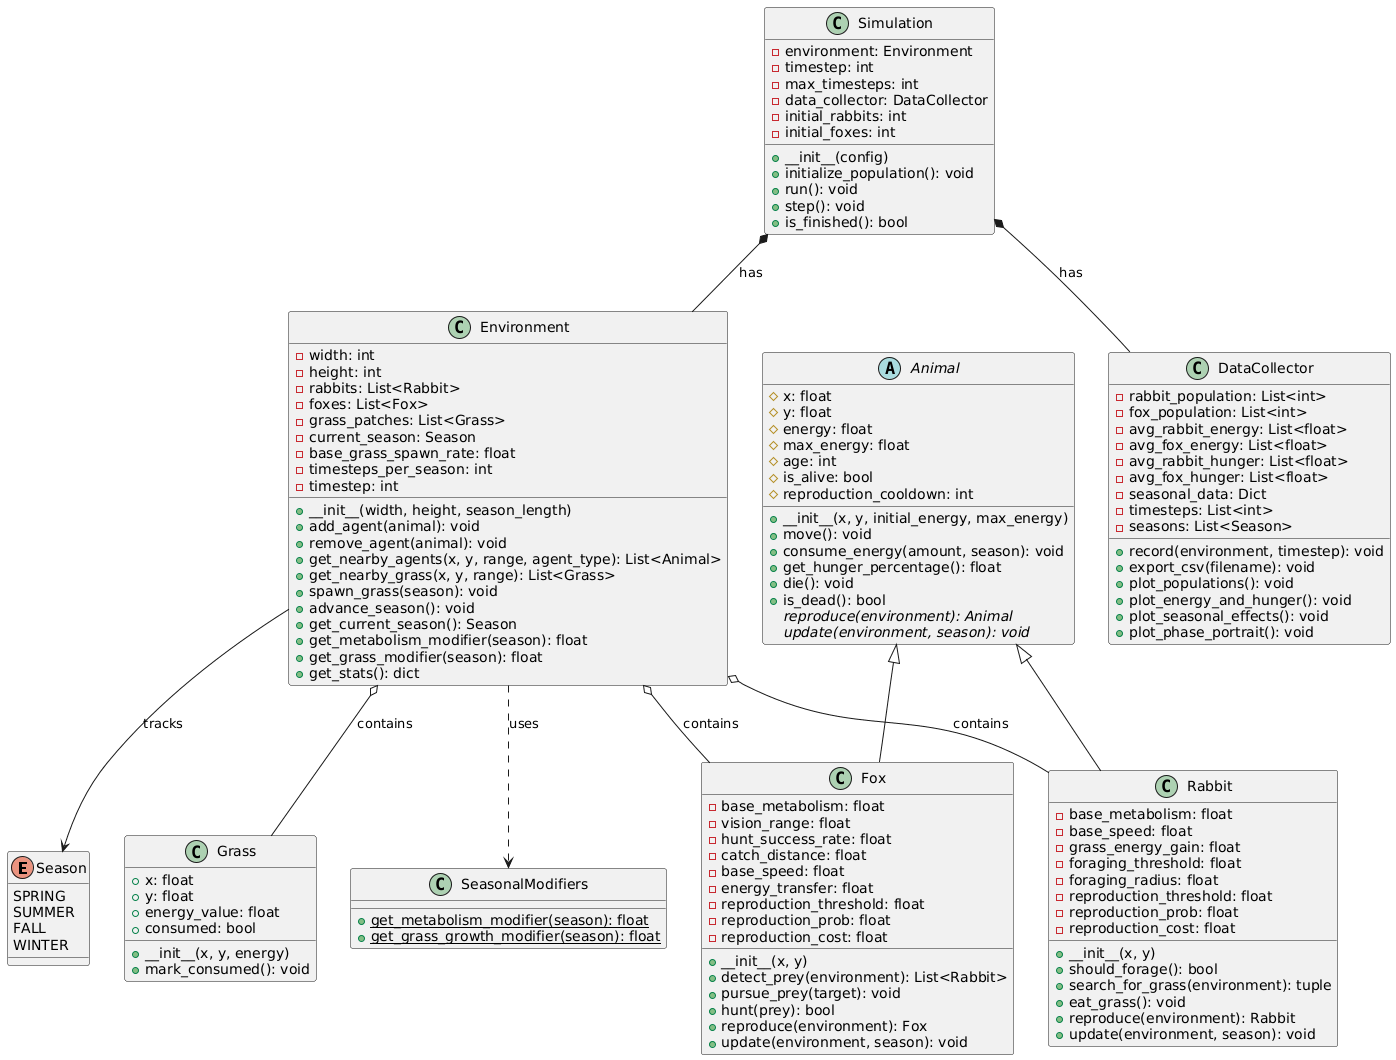
\includegraphics[width=0.8\textwidth]{classdiagram.png}
    \caption{UML Class Diagram of the simulation architecture.}
    \label{fig:classdiagram}
\end{figure}

\begin{figure}[H]
    \centering
    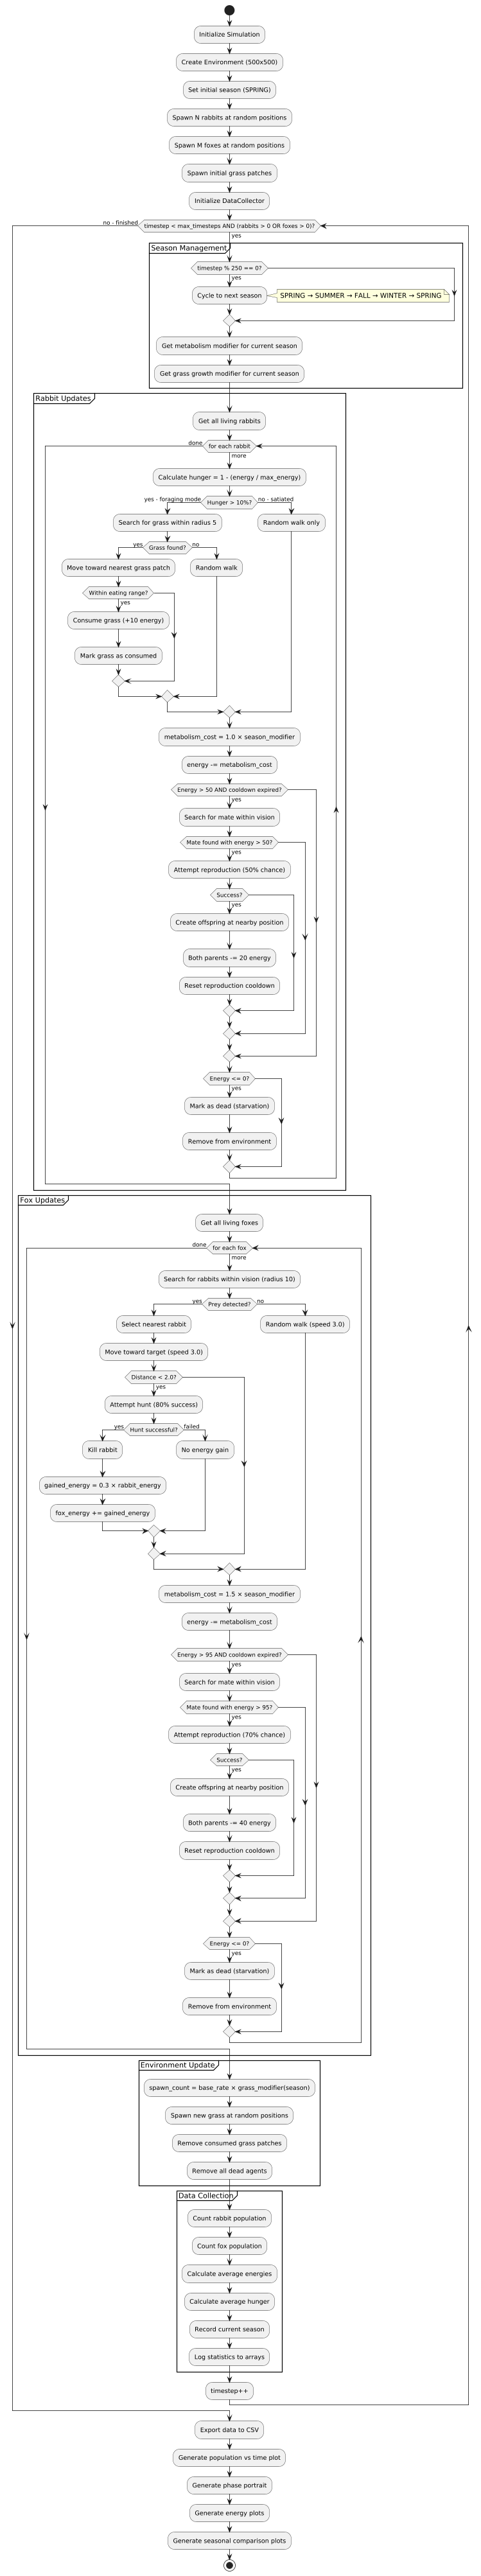
\includegraphics[width=0.8\textwidth]{behaviordiagram.png}
    \caption{Behavioral flowchart of agent decision making.}
    \label{fig:behaviordiagram}
\end{figure}

\subsection{Key Design Decisions}
A critical design decision was abandoning a discrete grid for spatial mapping. Instead, agents exist at floating-point coordinates, and neighbor discovery is handled by \texttt{scipy.spatial.KDTree}. This eliminates arbitrary grid-cell constraints and significantly improves the performance of distance queries. Additionally, a toroidal wrapping mechanism ensures the simulation area is continuous, preventing edge-accumulation artifacts.

% =============================================================================
\section{Implementation}
% =============================================================================

\subsection{Technologies Used}
The simulation is implemented in Python 3.13. Core libraries include NumPy for fast numerical operations, SciPy for KD-Tree spatial indexing, and Matplotlib for generating data visualizations.

\subsection{Core Algorithms}
\begin{itemize}
    \item \textbf{Hunger-Driven Foraging (Rabbits):} When energy drops below capacity, a rabbit queries the KD-Tree for the nearest grass patch within its foraging radius. If found, it moves towards it and consumes it upon arrival.
    \item \textbf{Predator Pursuit (Foxes):} Foxes query for the nearest rabbit within their vision radius. They adjust their trajectory to intercept the target.
    \item \textbf{Reproduction Mode:} When an animal's energy exceeds a species-specific threshold, it spawns an offspring with a portion of its energy, simulating biological reproduction costs.
\end{itemize}

\subsection{Challenges Overcome}
A major challenge was the performance bottleneck of spatial queries as populations grew. Early implementations using naive distance calculations scaled at (N^2)$, making large populations unfeasible. Integrating SciPy's KD-Tree reduced query times to (N \log N)$, allowing the simulation to handle thousands of entities smoothly.

% =============================================================================
\section{Experimental Setup}
% =============================================================================

\subsection{Simulation Parameters}
The baseline configuration (Run 001) is defined by:
\begin{itemize}
    \item Initial Populations: 100 Rabbits, 5 Foxes, 200 Grass patches.
    \item Grass Spawn Rate: 8 patches/step.
    \item Seasons: 250 steps each, with distinct multipliers. Spring (met=0.8, grs=2.0), Summer (met=1.0, grs=1.5), Fall (met=1.1, grs=0.7), Winter (met=1.4, grs=0.4).
\end{itemize}

\subsection{Scenarios Tested}
Ten distinct scenarios were executed to observe system behavior under varying conditions, including high initial populations (Runs 002, 003), resource scarcity/abundance (Runs 004, 005), extended duration (Run 006), harsh winter conditions (Run 007), mild uniform seasons (Run 008), high global density (Run 009), and alternate random seeds (Run 010).

\subsection{Data Collection Methods}
Data is collected continuously during the simulation. A time-series CSV records step-by-step population counts, births, consumption events, and active seasonal multipliers. A summary JSON captures aggregate statistics (e.g., max/min populations, total runtime), and a copy of the configuration JSON is archived for reproducibility.

% =============================================================================
\section{Results and Analysis}
\label{sec:results}
% =============================================================================

\subsection{Scenario Comparisons}

\begin{table}[H]
\centering
\caption{Summary of all 10 simulation runs}
\small
\begin{tabular}{clrrrrrcc}
\toprule
\textbf{Run} & \textbf{Description} & \textbf{Steps} & \textbf{Time (s)} &
\textbf{R\textsubscript{final}} & \textbf{F\textsubscript{final}} &
\textbf{R ext.} & \textbf{F ext.} \\
\midrule
001 & Baseline, all default parameters       & 1000 & 23.2 & 87  & 0  & No & Yes \\
002 & High rabbit count (200 rabbits)        & 1000 & 23.2 & 86  & 0  & No & Yes \\
003 & High fox count (20 foxes)              & 1000 & 16.4 & 81  & 0  & No & Yes \\
004 & Low initial grass (50 patches)         & 1000 & 21.4 & 90  & 0  & No & Yes \\
005 & High grass abundance (500 patches)     & 1000 & 38.2 & 133 & 0  & No & Yes \\
006 & Long run, 2 full years (2000 steps)    & 2000 & 52.2 & 82  & 0  & No & Yes \\
007 & Harsh winter (metabolism $\times.0)  & 1000 & 20.2 & 45  & 0  & No & Yes \\
008 & Mild seasons, uniform year-round       & 1000 & 18.7 & 161 & 10 & No & No  \\
009 & High entity count (300R, 15F, 300G)    & 1000 & 28.8 & 91  & 0  & No & Yes \\
010 & Different seed (seed=99), baseline     & 1000 & 20.4 & 89  & 0  & No & Yes \\
\bottomrule
\end{tabular}
\end{table}

\subsection{Predator-Prey Lag Effect}
In all runs, fox population peaks consistently lag behind rabbit population peaks by approximately 50 to 100 steps. This is the classic Lotka-Volterra delay: rabbits must first accumulate in large numbers before foxes have sufficient prey encounters to breed and grow their own population.

\begin{figure}[H]
    \centering
    \includegraphics[width=\textwidth]{run_001_population.png}
    \caption{Run 001 -- Baseline population dynamics. Fox peak lags rabbit peak by approximately 75 steps.}
    \label{fig:run001}
\end{figure}

\subsection{Seasonal Boom-Bust Cycles}
The baseline run (001) demonstrates a clear Spring boom where rabbits peak at 544 before foxes grow large enough (peak 54) to drive a crash. Rabbit populations partially recover in subsequent seasons before declining again through Winter as grass becomes scarce and metabolism costs rise. This multi-cycle damped oscillation is visible across the majority of runs.

\subsection{Harsh Winter vs. Mild Seasons}
Under doubled Winter metabolism (Run 007), rabbit populations reached a minimum of 17, the most severe decline of any run. Conversely, Run 008 (Mild Seasons) was the only run where foxes survived to the end of the simulation ( = 10$). With nearly uniform seasonal multipliers, the rabbit population never crashed hard enough to starve the fox population out, demonstrating stable coexistence.

\begin{figure}[H]
    \centering
    \includegraphics[width=\textwidth]{run_007_population.png}
    \caption{Run 007 -- Harsh winter conditions. Most severe population decline.}
\end{figure}

\begin{figure}[H]
    \centering
    \includegraphics[width=\textwidth]{run_008_population.png}
    \caption{Run 008 -- Mild uniform seasons. Stable coexistence achieved.}
\end{figure}

% =============================================================================
\section{Validation and Verification}
% =============================================================================

\subsection{Validation Methods Used}
The model was validated through sensitivity analysis and boundary condition testing. By running extreme scenarios (e.g., massive initial populations, zero predators), the system's behavior was checked against expected ecological outcomes.

\subsection{Evidence of Correctness}
Run 010 utilized a different random seed but produced macro-level dynamics nearly identical to the baseline (Run 001), confirming that the emergent behavior is robust and not an artifact of a specific random number sequence. Additionally, the observed phase lag between predator and prey peaks perfectly aligns with established Lotka-Volterra theory, verifying the fundamental correctness of the interaction logic.

\subsection{Limitations Acknowledged}
The simulation operates as a closed system with no immigration or emigration. This leads to permanent local extinction events (e.g., foxes dying out in 9 out of 10 runs). In real ecosystems, migration plays a key role in repopulating depleted areas.

% =============================================================================
\section{Discussion}
% =============================================================================

\subsection{Interpretation of Results}
The results clearly indicate that seasonal variation is the primary driver of population instability in this closed system. While the continuous spatial plane and localized vision allow for complex micro-interactions, the macro-level seasonal forcing dominates the long-term outcomes. The harsh winters reliably crash the prey population to levels that cannot sustain the predators, leading to predator extinction.

\subsection{Answered Research Questions}
We successfully demonstrated that continuous 2D spatial models can reproduce classic cyclical dynamics. Furthermore, we showed that extreme seasonal variations destabilize predator-prey cycles, while mild seasons promote stable coexistence.

\subsection{Practical Implications}
These findings highlight the vulnerability of specialized predators to environmental volatility. In conservation efforts, ensuring sufficient prey refuge or minimizing seasonal resource crashes is critical to maintaining apex predator populations.

% =============================================================================
\section{Conclusion and Future Work}
% =============================================================================

\subsection{Summary of Contributions}
This project successfully delivered a robust, high-performance continuous 2D agent-based simulation. The integration of spatial KD-Trees and dynamic seasonal environments provides a powerful framework for exploring complex ecological interactions beyond simple grid models.

\subsection{Lessons Learned}
A key lesson was the delicate balance required in parameter tuning. Small adjustments to metabolism or vision range drastically altered macro-level outcomes. Additionally, the transition from an (N^2)$ distance check to an (N \log N)$ KD-Tree query was a vital lesson in the importance of appropriate data structures for simulation scalability.

\subsection{Future Research Directions}
Future improvements should include open-system dynamics (migration), more complex cognitive behaviors for agents (e.g., flocking or pack hunting), and the introduction of a third trophic level (e.g., an apex predator or a competing prey species) to study more complex food web stability.

% =============================================================================
\section{References}
% =============================================================================
\begin{thebibliography}{9}
\bibitem{lotkavolterra}
Lotka, A. J. (1925). \textit{Elements of Physical Biology}. Williams and Wilkins, Baltimore.
\bibitem{scipy}
Virtanen, P., et al. (2020). SciPy 1.0: fundamental algorithms for scientific computing in Python. \textit{Nature Methods}, 17(3), 261-272.
\end{thebibliography}

\end{document}
